\documentclass[a4paper,10pt]{article}
\usepackage[english]{babel}
\usepackage[utf8]{inputenc}
\usepackage[T1]{fontenc}

\usepackage{tikz}
\usetikzlibrary{backgrounds}

\renewcommand\familydefault{\sfdefault}
\begin{document}
\pagestyle{empty}
\begin{center}
 \vfill
 \huge{\bf Log-In Information for this Course}
\end{center}
\vfil

\begin{center}
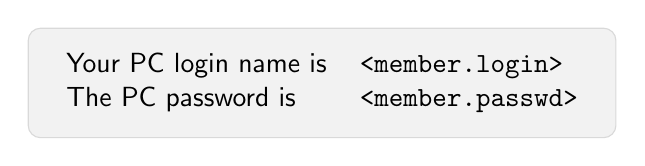
\begin{tikzpicture}[framed, background rectangle/.style={draw=black!15,fill=black!5,rounded corners=1ex}]
 
\node{

\begin{tabular}{ll}
Your PC login name is &   \texttt{\Var<member.login>} \\
The PC password is &      \texttt{\Var<member.passwd>}
\end{tabular}

};

\end{tikzpicture}
\end{center}

\vspace{1cm}

\begin{center}
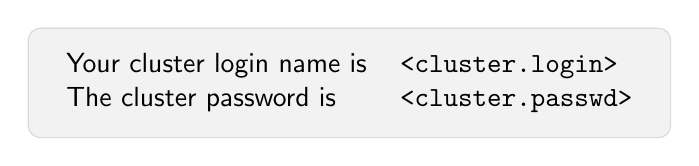
\begin{tikzpicture}[framed, background rectangle/.style={draw=black!15,fill=black!5,rounded corners=1ex}]
 
\node{

\begin{tabular}{ll}
Your cluster login name is &   \texttt{\Var<cluster.login>} \\
The cluster password is &      \texttt{\Var<cluster.passwd>}
\end{tabular}

};

\end{tikzpicture}
\end{center}

%TODO: fill in more info, once live-linux is available!

\vfil

Do not forget to log-out at the end of the course!

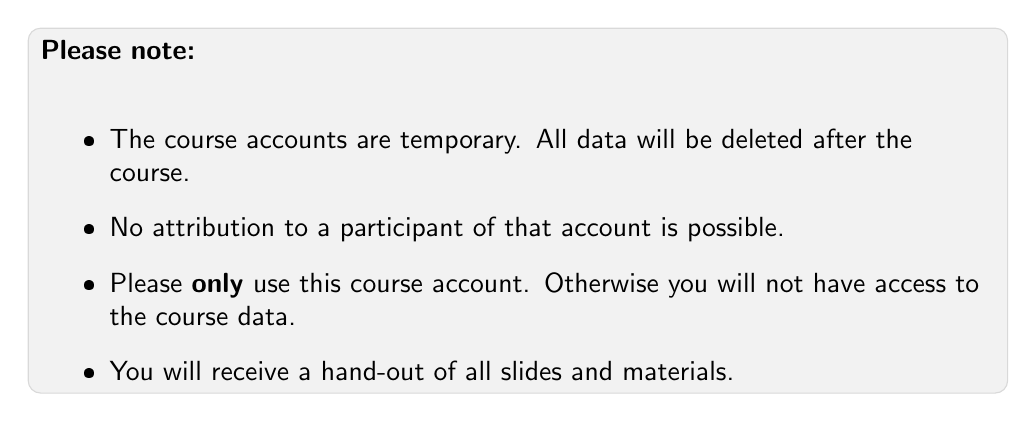
\begin{tikzpicture}[framed, background rectangle/.style={draw=black!15,fill=black!5,rounded corners=1ex}]
    \draw (current page.center) node[text width=\linewidth, inner sep=0cm] {
        \begin{minipage}[t]{\linewidth}
            \textbf{Please note:}\newline
            \begin{itemize}
              \item The course accounts are temporary. All data will be deleted after the course.
              \item No attribution to a participant of that account is possible.
              \item Please \textbf{only} use this course account. Otherwise you will not have access to the course data.
              \item You will receive a hand-out of all slides and materials. 
            \end{itemize}
        \end{minipage}
    };
\end{tikzpicture}

\vfill

%\begin{tikzpicture}[framed, background rectangle/.style={draw=black!15,fill=black!5,rounded corners=1ex}]
%    \draw (current page.center) node[text width=\linewidth, inner sep=0cm] {
%        \begin{minipage}[t]{\linewidth}
%            \textbf{Please scan:}\newline
%            Please await further instructions - we will take our time during the course to explain remote logins to our HPC-resources.\newline
%            Unsing your \texttt{FreeOTP} or \texttt{PrivacyIdea} application on your cellphone, add a security token using this QR-code:\newline
%            \begin{center}
%            \includegraphics[width=3.5cm]{\Var<member.qr>}
%            \end{center}
%        \end{minipage}
%    };
%\end{tikzpicture}
%\vfill

\end{document}

